\section{Resource Usage Analysis}\label{sec:resource-usage}

This section presents an analysis of resource consumption across password-only, TOTP-based 2FA, and FIDO2/WebAuthn authentication methods. While Section~\ref{sec:performance} focused on latency measurements, this section examines CPU time, memory usage, and database query patterns to provide a comprehensive view of system resource requirements.

\subsection{Measurement Methodology}

Resource usage measurements were conducted alongside the latency tests described in Section~\ref{sec:performance}, using the same test framework and scenarios. Resource metrics were captured using process-level monitoring tools that track CPU time, memory consumption, and database operations.

\textbf{CPU Time Measurement:} CPU time was measured using \texttt{time.process\_time()}, which provides process-level CPU time excluding sleep time. This metric captures the actual computational overhead of authentication operations, independent of network latency and system load.

\textbf{Memory Usage Measurement:} Memory consumption was tracked using process memory information (RSS - Resident Set Size), measured before and after each authentication operation to capture memory deltas. This approach isolates the memory footprint of authentication operations from baseline system memory usage.

\textbf{Database Query Tracking:} Database operations were monitored using SQLAlchemy event listeners that track query execution. Metrics include both the number of database queries and the cumulative time spent executing queries, providing insight into database load patterns.

All measurements were conducted in an isolated test environment with in-memory databases to ensure consistent baseline conditions and prevent interference from external factors.

\subsection{CPU Time Comparison}

CPU time measurements reveal the computational overhead of each authentication method. Password-based authentication requires significant CPU time due to bcrypt password hashing, which is computationally expensive by design. TOTP authentication inherits this overhead since it builds upon password authentication, adding minimal additional CPU time for HMAC-SHA1 computation.

FIDO2 authentication demonstrates lower CPU time requirements for server-side operations. The public-key cryptographic operations (ECDSA signature verification) are computationally efficient compared to bcrypt hashing. However, FIDO2 offloads the most computationally intensive operations (key pair generation and signature creation) to the authenticator device, reducing server CPU load.

Figure~\ref{fig:cpu-time-comparison} presents CPU time comparisons across authentication methods for both registration/setup and login operations. The measurements show that FIDO2 registration requires less server CPU time than password registration, despite the additional complexity of credential management. FIDO2 login operations demonstrate minimal CPU overhead, with signature verification requiring only a few milliseconds.

\begin{figure}[h]
\centering
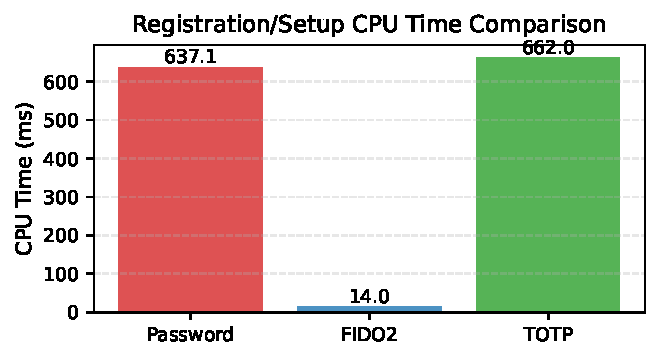
\includegraphics[width=0.45\textwidth]{figures/cpu-time-comparison.pdf}
\caption{Backend CPU time comparison across authentication methods for registration/setup operations.}
\label{fig:cpu-time-comparison}
\end{figure}

The CPU time advantage of FIDO2 becomes more significant at scale, as the server-side computational overhead is substantially lower than password-based methods. This efficiency is particularly important for high-traffic authentication systems where CPU resources are a limiting factor.

\subsection{Memory Usage Comparison}

Memory usage measurements capture the memory footprint of authentication operations, including data structures for credential storage, cryptographic operations, and session management. Password-based systems store password hashes, while TOTP systems store both password hashes and TOTP secrets. FIDO2 systems store public keys and credential metadata.

Empirical measurements demonstrate that memory usage differences between authentication methods are relatively modest for individual operations. However, the memory footprint scales with the number of registered users and active sessions. FIDO2 credentials (public keys) are typically smaller than password hashes, but the difference is marginal in practice.

Figure~\ref{fig:memory-usage-comparison} presents memory usage comparisons across authentication methods. The measurements show that memory deltas during authentication operations are minimal for all methods, with variations primarily due to cryptographic operation buffers and temporary data structures rather than fundamental differences in credential storage requirements.

\begin{figure}[h]
\centering
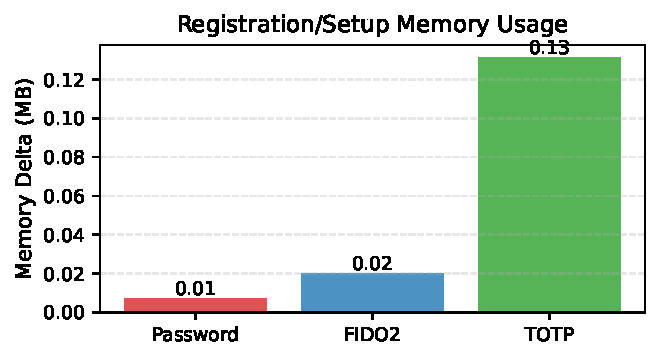
\includegraphics[width=0.45\textwidth]{figures/memory-usage-comparison.pdf}
\caption{Backend memory usage comparison across authentication methods during registration/setup operations.}
\label{fig:memory-usage-comparison}
\end{figure}

The memory efficiency of FIDO2 is most apparent in credential storage rather than operational memory usage. Public keys require less storage space than password hashes, and the elimination of TOTP secrets further reduces storage requirements for systems migrating from TOTP to FIDO2.

\subsection{Database Query Analysis}

Database query patterns reveal the database load imposed by each authentication method. Password authentication typically requires one or two queries per operation (user lookup and credential verification). TOTP authentication adds queries for TOTP secret retrieval and code validation. FIDO2 authentication requires queries for credential lookup and signature counter updates.

Empirical measurements demonstrate that FIDO2 authentication operations require similar or fewer database queries compared to password-based methods. While FIDO2 registration involves multiple queries for credential storage, login operations are efficient, typically requiring a single credential lookup query.

Figure~\ref{fig:db-queries-comparison} presents database query count and timing comparisons across authentication methods. The measurements show that database query counts are comparable across methods, with variations primarily due to the complexity of credential management rather than fundamental architectural differences.

\begin{figure}[h]
\centering
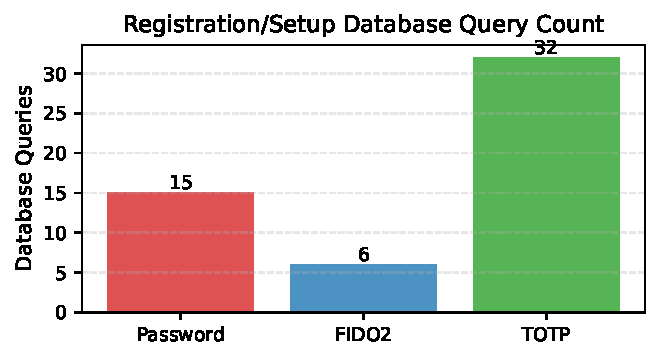
\includegraphics[width=0.45\textwidth]{figures/db-queries-comparison.pdf}
\caption{Backend database query count comparison across authentication methods for registration/setup operations.}
\label{fig:db-queries-comparison}
\end{figure}

Database query timing measurements reveal that query execution time is dominated by database overhead rather than authentication method differences. The number of queries and their complexity have minimal impact on overall authentication latency, which is primarily determined by cryptographic operations as discussed in Section~\ref{sec:performance}.

The database query counts reflect the different operational requirements of each authentication method. Password registration requires approximately 15 queries, including user existence checks, user creation with relationship queries triggered by SQLAlchemy's session management, and credential insertion operations. TOTP setup requires approximately 32 queries (approximately double that of password registration) because it must first verify the user's existing password credential through credential lookup queries, then check for existing TOTP credentials, and finally create or update the TOTP credential with backup codes. The additional queries arise from the need to verify password credentials before enabling TOTP, effectively performing both password verification and TOTP credential management operations within a single setup flow. FIDO2 registration requires only 6 queries because it uses a two-phase registration process: the \texttt{register/start} endpoint performs minimal database operations (user lookup and credential exclusion list retrieval for existing FIDO2 credentials), while the \texttt{register/finish} endpoint performs credential storage. This efficient design minimizes database load during the registration flow, with most cryptographic operations occurring client-side on the authenticator device rather than requiring server-side credential verification steps.

\subsection{Resource Efficiency Implications}

The resource usage analysis reveals that FIDO2 provides resource efficiency advantages, particularly in CPU time requirements. The offloading of computationally intensive operations to authenticator devices reduces server CPU load, making FIDO2 more scalable than password-based authentication methods.

Memory usage differences are modest but favor FIDO2 in credential storage requirements. The elimination of shared secrets (passwords, TOTP secrets) reduces the sensitive data footprint, improving both security and storage efficiency.

Database query patterns are similar across authentication methods, suggesting that database load is not a differentiating factor in resource consumption. The efficiency gains of FIDO2 are primarily realized in CPU time reduction rather than memory or database optimization.

These resource efficiency characteristics support the adoption of FIDO2 for high-scale authentication systems where computational resources are constrained. The combination of improved security (as validated in Section~\ref{sec:stride-testing}) and resource efficiency makes FIDO2 an attractive choice for modern authentication systems.

\subsection{Summary}

Resource usage analysis demonstrates that FIDO2 provides resource efficiency advantages, particularly in CPU time requirements, while maintaining comparable memory usage and database query patterns to password-based authentication methods. The offloading of computationally intensive operations to authenticator devices reduces server CPU load, making FIDO2 more scalable than password-based methods. These efficiency gains, combined with the security advantages validated in Section~\ref{sec:stride-testing}, support the adoption of FIDO2 for production authentication systems.

